\part{\LaTeX}

\chapter{General}

\section{Glossaries}

\Glspl{glossary} are being defined as ``\textit{an alphabetical list of words related to a specific subject, text, or dialect, with explanations; a brief dictionary}". To automate \glspl{glossary} generation and maintenence, \LaTeX\ uses a package called: \textbf{\glspl{glossary}}. Like in most cases, it is sometimes desired to specify additional \glspl{parameter} to the package, e.g. \textit{acronym}, \textit{toc}, \textit{section=section}. Which will be explained later in this section.\\

Before processing any code two things have to be mentioned. One: \glspl{glossary} package require \textbf{\href{https://www.perl.org/}{Perl}} interpreter to be present at the machine. Two: the package requires custom compilation scheme in order to take effect. Unfortunately there is no preset built into \textbf{\href{https://www.xm1math.net/texmaker/}{TeXMaker}} environment for a compilation scheme that will proces glossaries. A custom command \gls{pipeline} has to be configured manually.

\begin{figure}[H]
\centering
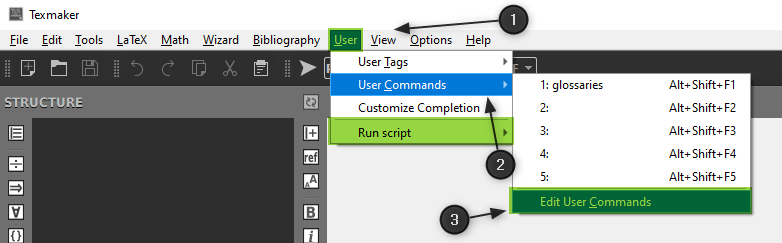
\includegraphics[scale=0.6]{content/LaTeX/figures/user_command_glossaries_marked.png}
\caption{Location of \textbf{Edit User Commands} button in \textbf{\href{https://www.xm1math.net/texmaker/}{TeXMaker}} environment}
\end{figure}

In order to define the custom command \gls{pipeline}, go to: \textbf{User} -> \textbf{User Commands} -> \textbf{Edit User Commands} and type below code into \textbf{command} field:
%\vspace{-0.5em} --------------------------------------------------------------------
\begin{verbatim}
pdflatex -synctex=1 -interaction=nonstopmode %.tex | makeglossaries % | pdflatex 
-synctex=1 -interaction=nonstopmode %.tex | "C:/Program Files (x86)/Adobe/Acrobat
Reader DC/Reader/AcroRd32.exe" %.pdf
\end{verbatim}

\begin{figure}[H]
\centering
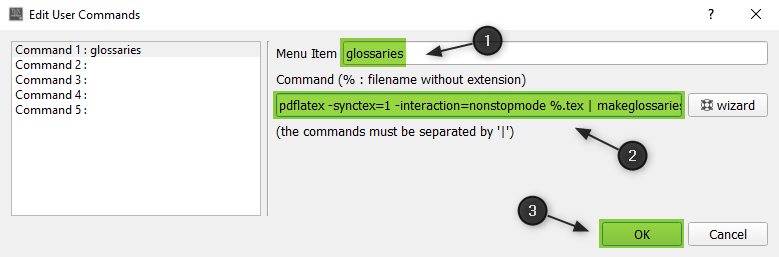
\includegraphics[scale=0.6]{content/LaTeX/figures/custom_command_marked.png}
\caption{Layout of \textbf{Edit User Commands} window in \textbf{\href{https://www.xm1math.net/texmaker/}{TeXMaker}} environment}
\end{figure}

Pipe symbol is used to chain commands. Words preceded by pause: ``-'' are \glspl{parameter} passed to commands, which are words without any additions, placed at the beginning of every part - right after pipe or at the very beginning. Disassembly of this chain of commands allows to differentiate four differents parts here:
\begin{enumerate}
\item Generate \textbf{.pdf} file from the \textbf{.tex} file
\item Generate \glspl{glossary}
\item Generate \textbf{.pdf} file from the \textbf{.tex} file
\item Display \textbf{.pdf}
\end{enumerate}

There are two types of entries that \gls{glossary} package provides by default:
\begin{itemize}
\item \glspl{glossary}
\item acronyms
\end{itemize}

\Glspl{glossary} are being defined in the preamble after \texttt{\bs makeglossaries} command that has to be put before any of the entries. Syntax of an \gls{glossary} and acronym entry is as shown below.

\begin{figure}[H]
\centering
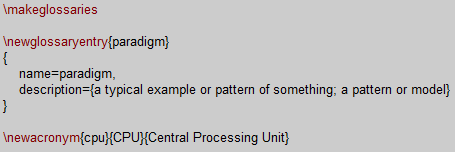
\includegraphics[scale=1.0]{content/LaTeX/figures/glossary_definition.png}
\caption{Commands used to define \glspl{glossary} and acronyms}
\label{fig:glossary_definition}
\end{figure}

To print a list of \glspl{glossary}, \texttt{\bs printglossary} command is used. For an entry to be printed on the list, at least one reference to it in the text is needed. Otherwise even if defined in the preamble, the entry won't be printet on the list.

\begin{figure}[H]
\centering
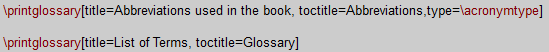
\includegraphics[scale=1.0]{content/LaTeX/figures/printglossary.png}
\caption{Commands used to print \gls{glossary} and acronym list}
\label{fig:printglossary}
\end{figure}

By default a list containing both \glspl{glossary} and acronyms is printed. As shown later on figure \ref{fig:usepackage_glossaries} \gls{parameter} \texttt{acronym} can be provided while invoking the package use, that allows to print separate list for acronyms and \glspl{glossary}. To print the separate list for acronyms specify \texttt{type=\bs acronymtype} attribute in a separate \texttt{\bs printglossary} call as shown on figure \ref{fig:printglossary}, which also illustrate, how a custom title\footnote{Title displayed in the text} as well as token title\footnote{Title displayed in table of content} can be set. To allow \gls{glossary} table to be included in table of contents an additional parameters: \texttt{toc} and \texttt{section=section} are needed when invoking \textbf{\glspl{glossary}} package as shown on picture \ref{fig:usepackage_glossaries}.

\begin{figure}[H]
\centering
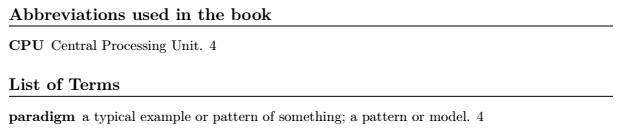
\includegraphics[scale=0.8]{content/LaTeX/figures/glossary_types.png}
\caption{Lists of acronyms and glossaries generated separately with use of \textbf{acronym} parameter for \textbf{\glspl{glossary}} package, that allows for separate list for acronyms to be printed}
\end{figure}

To reference a \gls{glossary} or acronym, several commands are used.

\begin{figure}[H]
\centering
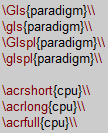
\includegraphics[scale=1.0]{content/LaTeX/figures/reference_glossaries.png}
\caption{Commands used to reference \glspl{glossary} and acronyms}
\end{figure}

Each entry can be referenced in several ways. Plural and singular forms as well as upper case and lowercase versions are avaliable for \glspl{glossary}. Acronym references differ from each other by level of detail printed.

\begin{figure}[H]
\centering
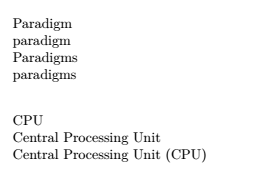
\includegraphics[scale=1.0]{content/LaTeX/figures/glossary_calls.png}
\caption{Examples of \glspl{glossary} and acronyms references}
\end{figure}

\begin{figure}[H]
\centering

\includegraphics[scale=1.0]{content/LaTeX/figures/usepackage_glossaries.png}
\caption{Command used to invoke the use of \textbf{glossaries} package with additional parameters passed to it}
\label{fig:usepackage_glossaries}
\end{figure}

There are many more options regarding to \gls{glossary} package, i.e. commands used to customize display of the \gls{glossary}, enable sorting, create custom \glspl{glossary}, put alternative text in references to a \gls{glossary}, define custom spelling for plural form, etc. You can find them on \acrshort{ctan} \href{https://www.ctan.org/pkg/glossaries}{website}~\cite{ctan_glossaries}.

\section{Bibliography}

In order to automate the process, make it more flexible and easily maintainable, there is a bibliography processor shipped with \Gls{miktex}, called \textbf{\Gls{bibtex}}. In general \textbf{\Gls{bibtex}} is considerd to be standalone tool, but in real life practice, it has very few uses, beside being bibliography management system for \LaTeX distributions. Thus it's very convinient to include it in \Gls{miktex} package by default.

\Gls{bibtex} itself alows to create citations to specified bibliography. It also contains built in bibliography listing functionality with predefined styles, that can be overriden.

\begin{figure}[H]
\centering
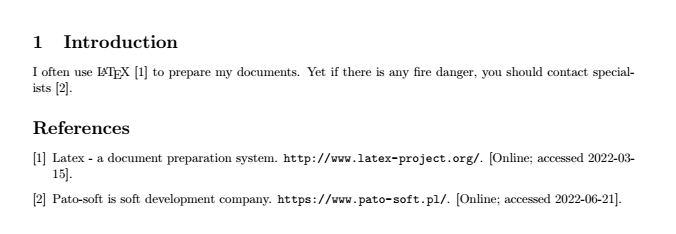
\includegraphics[scale=0.8]{content/LaTeX/figures/biblio_outcome.png}
\caption{An example showing default style of bibliography listing with citations generated by \gls{bibtex}}
\label{fig:bibliography_example}
\end{figure}

Bibliography items are stored in files with \textbf{\gls{bib}} extension, which are organized as a key-value dictionary. There is a set of allowed key values, to be used in a bibliography entry. There are no order restrictions on which key should be specified first, although it is usualy good to folow some convenctions like specifying the title first.

\begin{figure}[H]
\centering
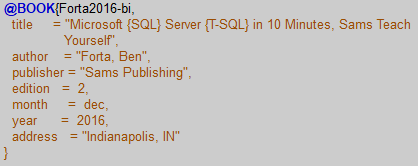
\includegraphics[scale=0.9]{content/LaTeX/figures/biblio_example.png}
\caption{Structure of a bibliography item entry in a \gls{bib} file}
\label{fig:biblio_example}
\end{figure}

\begin{figure}[H]
\centering
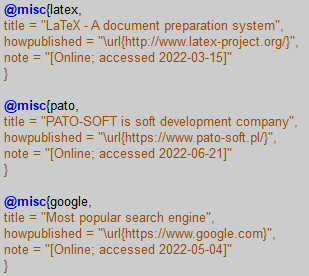
\includegraphics[scale=0.9]{content/LaTeX/figures/biblio_bib.png}
\caption{Example of website entries in a \textbf{.bib} file}
\label{fig:biblio_websites}
\end{figure}

By default only entries that have been cited are printed in the bibliography listing. This behavious can be changed by using \texttt{\bs nocite\{*\}} command. It accepts keys as parameters, to print certain entries. Using asterix results in printing all results.

\begin{figure}[H]
\centering
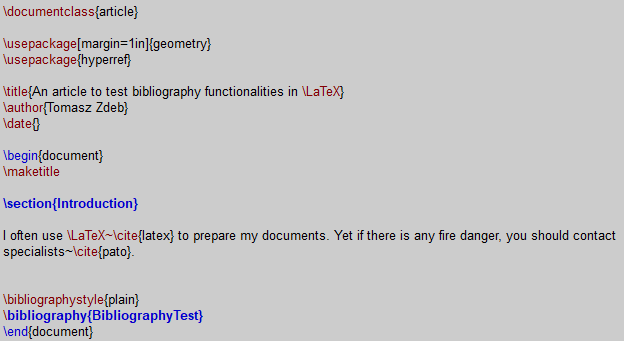
\includegraphics[scale=0.9]{content/LaTeX/figures/biblio_latex.png}
\caption{Example showing how to use citing in the document}
\label{fig:biblio_usage}
\end{figure}

Bibtex compilation pipeline consists of several compilation steps. By processing \textbf{.bib} files, \textbf{.bbl} files are being produced, which are the direct source of content for \textbf{pdflatex}.

\begin{figure}[H]
\centering
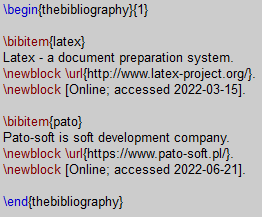
\includegraphics[scale=0.9]{content/LaTeX/figures/biblio_bbl.png}
\caption{Example of a \textbf{.bbl} file structure}
\label{fig:biblio_bbl_example}
\end{figure}

Some quick guides, as well as some converters can be found \href{https://www.bibtex.com/g/bibtex-format/}{here} and \href{https://www.overleaf.com/learn/latex/Bibliography_management_with_bibtex}{here}. Additional information can be found \href{https://tug.org/bibtex/}{here}.\\

Advanced users may want to create a bibliography after each parto or chapter. Detailed guide on how to achieve such effets can be found \href{https://tex.stackexchange.com/questions/229846/different-bibliographies-for-each-chapter-with-shared-references}{here}

\section{Listing environments}

\subsection{Enumerate}

\begin{figure}[H]
\centering
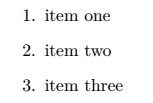
\includegraphics[scale=0.8]{content/LaTeX/figures/enumerate_outcome_example.png}
\caption{Example of an enumerate environment}
\label{fig:enumerate_outcome_example}
\end{figure}

Source code:

\begin{Verbatim}
\begin{enumerate}
  \item item one
  \item item two
  \item item three
\end{enumerate} 
\end{Verbatim}

\subsection{Itemize}

\begin{figure}[H]
\centering
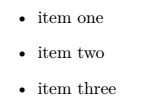
\includegraphics[scale=0.8]{content/LaTeX/figures/itemize_outcome_example.png}
\caption{Example of an itemize environment}
\label{fig:itemize_outcome_example}
\end{figure}

Source code:

\begin{Verbatim}
\begin{itemize}
  \item item one
  \item item two
  \item item three
\end{itemize} 
\end{Verbatim}

\subsection{Description}

\begin{figure}[H]
\centering
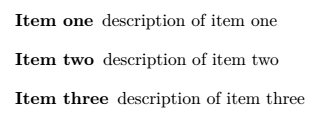
\includegraphics[scale=0.8]{content/LaTeX/figures/description_outcome_example.png}
\caption{Example of an description environment}
\label{fig:description_outcome_example}
\end{figure}

Source code:

\begin{Verbatim}
\begin{description}
  \item[Item one] description of item one
  \item[Item two] description of item two
  \item[Item three] description of item three
\end{description} 
\end{Verbatim}

\section{Where to inser captions and labels}
\fbox{\textcolor{red}{remember to surround tables, figures etc. in their wrapper floatin environments like figure, table etc. and add the caption and label}}
\section{How to avoid a line break}
\fbox{\textcolor{red}{to instruct \LaTeX no to break line between some content use tilde, e.g. no\textasciitilde line\textasciitilde break}}
\section{How to generate tilde}
\fbox{\textcolor{red}{FINISH THIS CHAPTER}}
\section{Differences between ref and hred referencing}
\fbox{\textcolor{red}{FINISH THIS CHAPTER}}
\section{MikTeX standard files}
\fbox{\textcolor{red}{FINISH THIS CHAPTER}}
\begin{verbatim}
C:\Program Files\MiKTeX\tex\latex\base
\end{verbatim}
\section{TO DOs}
\fbox{\textcolor{red}{Add list of tables and list of figures to the table}}\\
\fbox{\textcolor{red}{Add bibliography to the list of contents}}\\
\fbox{\textcolor{red}{Add non numbered chapter: acronyms and glossaries to table of contents}}\\
\fbox{\textcolor{red}{Go through the whole document and add lacking glossary/acronym entries}}\\
\fbox{\textcolor{red}{Go through the whole document and add lacking bibliography entries}}\\
\fbox{\url{http://www.peteryu.ca/tutorials/publishing/latex_captions}}\\
\fbox{\url{https://tex.stackexchange.com/questions/229846/different-bibliographies-for-each-chapter-with-shared-references}}\\
\fbox{\url{https://ctan.org/pkg/multirow}}\\
\fbox{\url{https://dictionary.cambridge.org/pl/dictionary/english/glossary}}\\
\fbox{\url{https://tex.stackexchange.com/questions/17653/how-to-list-all-bibliography-entries-without-citing}}\\
\fbox{\url{https://www.overleaf.com/learn/latex/Algorithms}}\\
\fbox{\url{https://tex.stackexchange.com/questions/1669/resuming-a-list}}\\

